\documentclass[12pt,A4paper
english, % ngerman for German
singlespacing, % Single line spacing, alternatives: onehalfspacing or doublespacing
%draft, % Uncomment to enable draft mode (no pictures, no links, overfull hboxes indicated)
%nolistspacing, % If the document is onehalfspacing or doublespacing, uncomment this to set spacing in lists to single
%liststotoc, % Uncomment to add the list of figures/tables/etc to the table of contents
%toctotoc, % Uncomment to add the main table of contents to the table of contents
parskip, % Uncomment to add space between paragraphs
%nohyperref, % Uncomment to not load the hyperref package
headsepline, % Uncomment to get a line under the header
]{article}

\usepackage[colorlinks=true,
            linkcolor=blue,
            urlcolor=blue,
            citecolor=gray]{hyperref}
            
\setcounter{secnumdepth}{3}
\usepackage[utf8]{inputenc} % Required for inputting international characters
\usepackage[T1]{fontenc} % Output font encoding for international characters
\usepackage[graphicx]{realboxes}
%\usepackage[sort,square,numbers]{natbib}

%\pdfoutput=1
\usepackage{cite}
\usepackage{hyperref}
\usepackage{graphicx}
\usepackage{subfig}
\usepackage{rotating}
\usepackage{booktabs}
    \usepackage{pdflscape}
    \usepackage{amsmath}
    \usepackage{caption}
    \usepackage{enumerate} 
    \usepackage{cancel}
    \usepackage{longtable}
    \usepackage[toc,page]{appendix}
    \usepackage{slashed}
    \usepackage{etoolbox} % provides \patchcmd macro1
    \makeatletter % modify the "headings" page style
    \patchcmd{\ps@headings}{{\slshape
ightmark}\hfil	hepage}{	hepage\hfil}{}{}
    \makeatother
    \usepackage{authblk}
    
\usepackage{color}
\usepackage{subfigure}
\usepackage{subcaption}

\textwidth 170mm
\textheight 220mm
\oddsidemargin -5mm
\evensidemargin 5mm
\topmargin -16pt
\usepackage{multirow}
\renewcommand\arraystretch{1.7} 

\newcommand{\amc}{{\sc MadGraph5\textunderscore}a{\sc MC@NLO}}

\newcommand{\MHT}{ $\slashed H _T$}
\newcommand{\HT}{ $ H _T$}

\newcommand{\NJETS}{$N_{jet}$}
\newcommand{\NB}{$n_b$}

\newcommand{\MAD}{\texttt{MadAnalysis 5}}

\begin{document}
\hypersetup{%
  colorlinks = true,
  linkcolor  = blue
}


\title{MadAnalysis5 validation for the recasting of CMS-SUS-16-033}
\author{Federico~Ambrogi}

\renewcommand{\thefootnote}{\arabic{footnote}}

\maketitle
{\it University of Vienna, Faculty of Physics, Bolzmanngasse 5, A-1090 Wien, Austria 
\\

email: federico.ambrogi88@gmail.com\\[2mm]
}

\begin{abstract}
This document constitutes the validation note for the \MAD~\cite{Conte:2012fm,Conte:2014zja,Dumont:2014tja} implementation of the analysis CMS-SUS-16-033 \cite{Sirunyan:2017cwe} \textit{``Search for supersymmetry in multijet events with missing transverse momentum in proton-proton collisions at 13 TeV"} by the CMS Collaboration. The recast code can be found on \texttt{INSPIRE}\cite{code}.
\end{abstract}

\tableofcontents

\clearpage
\section{CMS-SUS-16-033 Analysis Description}
The analysis CMS-SUS-16-033\cite{Sirunyan:2017cwe} is designed for the search of Supersymmetric (SUSY) particles decaying in the `all hadronic' final state. The data analyzed, that corresponds to an integrated luminosity of $35.9 \ fb^{-1}$, was collected with proton-proton collisions at a center of mass energy of 13 TeV. 
\\

The search is performed using four main kinematic variables: the light and b-tagged jets (i.e. jets originating from the hadronization of a bottom quark), the hadronic transverse energy ($H_T$) and the missing transverse energy ($\slashed {H}_T$). 
\\

All the information as well as the validation material used in the following is publicly available on the official wiki page of the analysis \footnote{\url{http://cms-results.web.cern.ch/cms-results/public-results/publications/SUS-16-033/index.html}}. 

\paragraph{Events selection}
\newline
The selection of events requires no isolated leptons (electrons or muons), and the $p_T$ of the lepton determine the isolation radius:
\begin{itemize}
\item $\Delta R < 0.2 $ if $p_T < 50$ GeV ; \
\item $\Delta R = 10$ GeV $ / p_T $ for $ 50 \leq p_T \leq  200$ GeV ; \
\item $\Delta R = 0.05$ if $p_T >200$ GeV.
\end{itemize}
\\
 
The isolation variable $I_l$ is defined as:
\begin{equation*}
I_l = \frac{\sum _{< \Delta R} p_T(h,c) + p_T(h,n) + p_T(\gamma) } {p_T(l) }
\end{equation*}
 
where the sum at the numerator includes the scalar $p_T$ of the charged (h,c) and neutral (h,n) hadrons and the photons. The sum is performed over all the objects included in a radius  $\Delta R = \sqrt{ (\Delta \phi)^2 + (\Delta \eta)^2 }$ around the lepton direction. 
\\
 
Electrons and muons are considered isolated if $I_e <$0.2 and $I_{\mu} <$0.1 respectively. The analysis also vetoes isolated tracks, with again isolation requirements depending on the type and momentum of tracks being considered.
\\
 
Coming to jets, the variable $H_T$ is defined as the scalar sum of the $p_T$ of the signal jets:
\begin{equation}
H_T = \sum_{\substack{jets (p_T> 30 GeV})}  | \vec{p}_T | 
\end{equation}
\\
where only the jets with $p_T>30 \ GeV$ and $|\eta| < 2.4$ are used.
The variable $\slashed {H}_T$ is instead defined as the jets momenta vectorial sum:
\begin{equation}
\slashed {H}_T = | \vec{\slashed {H}}_T | =  \left | \ \sum_{\substack{jets (p_T> 30 GeV)}}  \vec{p}_T \ \right |
\end{equation}
\\
for jets with $|\eta| < 5.0$ . 
\\

Additional event selections require an angular separation of the azimuthal angle $\Delta \phi(\vec{\slashed{H}_T},\vec{p_T})$  between the jets up to the fourth highest $p_T$ jet: the first two-highest-$p_T$ jets must satisfy $\Delta \phi>$0.5, while the 3rd and 4th-highest, if present in the event, must satisfy $\Delta \phi>$0.3.
\\

\section{Samples Generation}
The results of the analyses are interpreted in the context of simplified models spectra, and detailed information (cutflow tables, kinematic distributions and events yields) are provided for several benchmark points, for gluino and squark pair production. No specific information from the CMS collaboration regarding the samples production is available. 
\\

The SUSY signal samples were produced using \amc~\cite{Alwall:2011uj,Alwall:2014hca} for the hard scattering process, while the hadronization and showering were performed using {\sc PYTHIA 6.4} \cite{Sjostrand:2006za}. Samples were generated with up to one additional parton. The MLM merging scheme was chosen, with parameters $(XQcut,Qcut)=(30,65),(30,160)$ for the case of squark and gluino production respectively.

After the merging procedure, around 100.000 events were passed to the detector simulations in order to ensure statistical robustness. 
\\

The CMS detector simulation was performed using the {\sc Delphes 3.4.0}\cite{deFavereau:2013fsa} fast simulation tool; the CMS card was tuned according to the b-tagging efficiency fitted formula \footnote{https://twiki.cern.ch/twiki/bin/view/CMSPublic/SUSICHEP2016ObjectsEfficiency} and b-tagging mis-identification rate as provided\footnote{ \url{
https://twiki.cern.ch/twiki/pub/CMSPublic/BTV13TeVICHEP2016/xSig\_4\_0\_AErr\_2\_CSVv2L\_0\_0\_2\_4.pdf
}} by the CMS collaboration for 13 TeV data.
\\

Jets were clustered using {\sc FastJet} 3.2.1 \cite{Cacciari:2011ma}, with the $anti-k_T$ \cite{Cacciari:2008gp} algorithm, with $\Delta R = 0.4$ .
\\

\clearpage
\section{\MAD~ Validation}

The following list of simplified models were tested and validated:
\begin{itemize}
\item \textit{T2qq}: $\tilde{q}\tilde{q}, \tilde{q} \rightarrow q  \tilde{\chi}_{1}^{0}$ for  ($m_{\tilde{q}} , m_{\tilde{\chi}_1^0}) = (1000,800) , (700,400)$ ;
\item \textit{T2bb}: $\tilde{b}\tilde{b}, \tilde{b} \rightarrow b  \tilde{\chi}_{1}^{0}$ for ($m_{\tilde{b}} , m_{\tilde{\chi}_1^0}) = (650,1) , (500,300)$ ;
%\item \textit{T2tt}: $\tilde{t}\tilde{t}, \tilde{t} \rightarrow t  \tilde{\chi}_{1}^{0}$ for ($m_{\tilde{t}} , m_{\tilde{\chi}_1^0}) = (700,50) , (300,200)$ ;
\item \textit{T1qqqq}: $\tilde{g}\tilde{g}, \tilde{g} \rightarrow qq \tilde{\chi}^{0}_{1}$ for ($m_{\tilde{g}} , m_{\tilde{\chi}_1^0}) = (1400,100) , (2000,800)$ ;
\item \textit{T1bbbb}: $\tilde{g}\tilde{g}, \tilde{g} \rightarrow bb \tilde{\chi}^{0}_{1}$ for($m_{\tilde{g}} , m_{\tilde{\chi}_1^0}) = (1500,100) , (1000,900)$ ;
%\item \textit{T1tttt}: $\tilde{g}\tilde{g}, \tilde{g} \rightarrow tt \tilde{\chi}^{0}_{1}$ for ($m_{\tilde{g}} , m_{\tilde{\chi}_1^0}) = (1500,100) , (1200,800)$ ;
%\item T5VV: $\tilde{g}\tilde{g}, \tilde{g} \rightarrow qq(\tilde{\chi}^{\pm}_{1}/ \tilde{\chi}^{0}_{2})\rightarrow qq (W/Z)\tilde{\chi}^{0}_{1}$ for ($m_{\tilde{g}} , m_{\tilde{\chi}_1^0}) = (1400,100) , (1200,800)$ ;
\end{itemize}
\\

For each simplified model in the list above, the preselection cut flows, the kinematic histograms for the \NJETS~,\NB~,\HT~and \MHT~variables, and the signal yield for the aggregated signal regions, are validated. 
\\

The reference cross section for gluino,squark and sbottom production were taken from the LHC SUSY working group \footnote{\url{https://twiki.cern.ch/twiki/bin/view/LHCPhysics/SUSYCrossSections}}, and used to normalize the kinematic distributions and to calculate the yields in the aggregated signal regions.
\\

The kinematic distributions are obtained right after the preselection cuts: all the cuts are applied but the one involving the variable shown in the plot. The histogram data obtained from \MAD~are weighted with the total luminosity, production cross section and divided by the number of generated events. The same normalization applies when evaluating the yields in the aggregated signal regions.

\clearpage
\subsection{T2qq Simplified Model}
\begin{figure}[ht!] \begin{center}
\subfigure {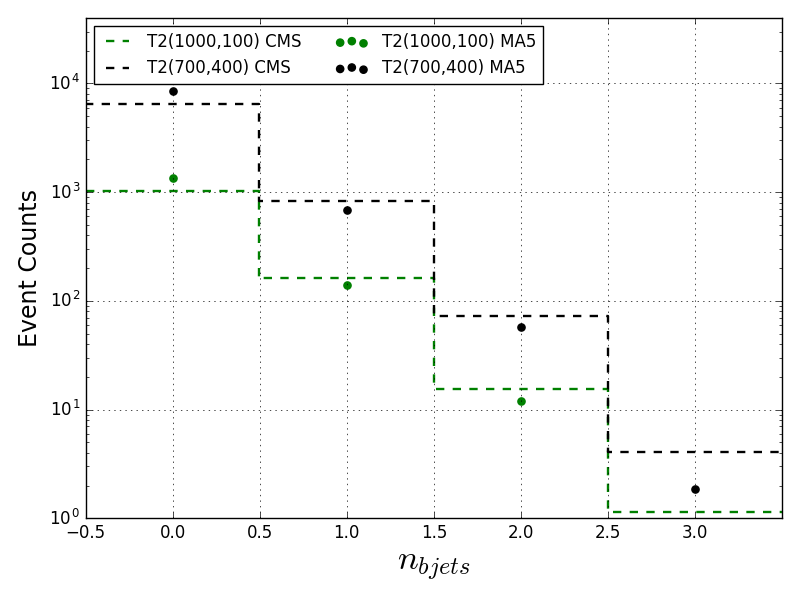
\includegraphics[width=0.49\textwidth]{PLOTS/Squarks_bJets_Pre.png}}
\subfigure {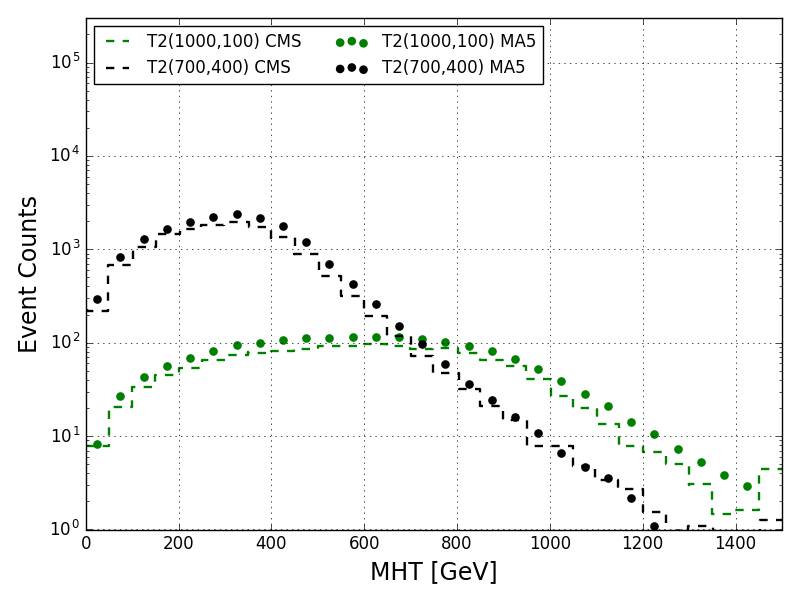
\includegraphics[width=0.49\textwidth]{PLOTS/Squarks_MHT_Pre.png}}
\subfigure {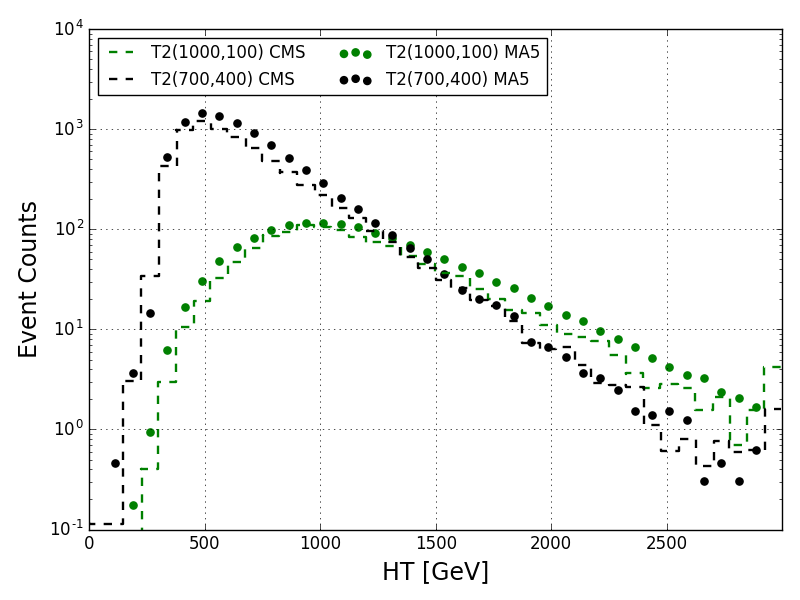
\includegraphics[width=0.49\textwidth]{PLOTS/Squarks_HT_Pre.png}}
\subfigure {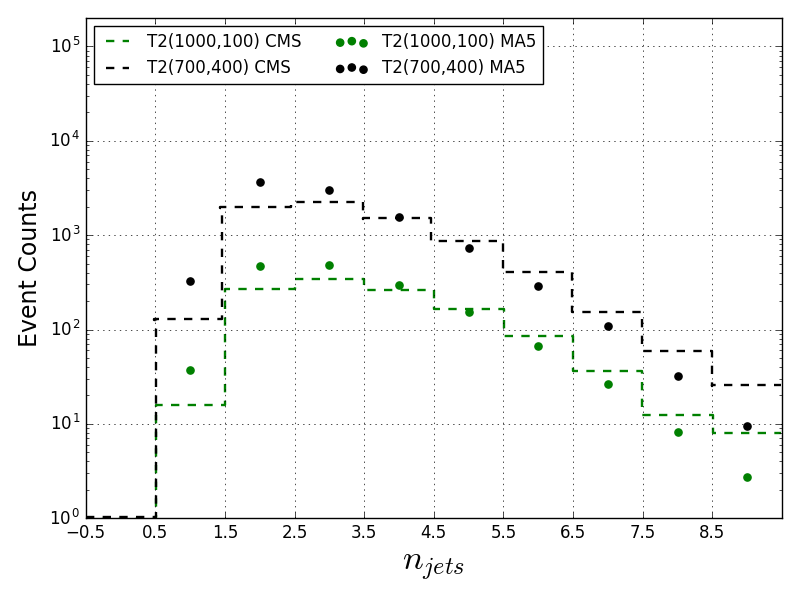
\includegraphics[width=0.49\textwidth]{PLOTS/Squarks_nJets_Pre.png}}
\end{center}
\caption{Kinematic distributions for the T2qq simplified models.}
\end{figure}

\clearpage
\begin{table}
\renewcommand{\arraystretch}{1.5}
\centering
\scriptsize
\begin{tabular} {  c | c | c | c | c | c  ||  c | c | c | c | c  }  
\multicolumn{1}{ c }{ }  &  \multicolumn{5}{ c }{ \textbf{T2qq(700,400)}} & \multicolumn{5 }{c}{ \textbf{T2qq(1000,100)}} \\ \toprule
 \multicolumn{1}{ c }{ } &  \multicolumn{3}{c}{Absolute} & \multicolumn{2}{c}{Drop[$\%$]} & \multicolumn{3}{c}{Absolute} & \multicolumn{2}{c}{Drop[$\%$]} \\ \toprule \toprule
 \textbf{Cut} & \textbf{MA5} & \textbf{CMS} & \textbf{Diff(}\%\textbf{)} & \textbf{MA5} & \textbf{CMS} & \textbf{MA5} & \textbf{CMS} & \textbf{Diff(}\%\textbf{)} & \textbf{MA5} & \textbf{CMS} \\ 
 \toprule \toprule 
\NJETS$\ge$2 &  96.18 & 98.00 & 1.86 & -3.82 & -2.00 &  97.82 & 98.90 & 1.09 & -2.18 & -1.10\\ 
\HT~$>$300 &  87.85 & 91.30 & 3.78 & -8.66 & -6.84 &  97.12 & 98.60 & 1.50 & -0.72 & -0.30\\ 
\MHT~$>$300 &  43.63 & 43.80 & 0.39 & -50.34 & -52.03 &  79.16 & 80.00 & 1.04 & -18.49 & -18.86\\ 
NoIsoMuons &  43.63 & 43.80 & 0.39 & 0.00 & 0.00 &  79.16 & 79.90 & 0.92 & -0.00 & -0.12\\ 
NoMuonsTracks &  43.61 & 43.70 & 0.20 & -0.04 & -0.23 &  79.14 & 79.80 & 0.82 & -0.03 & -0.13\\ 
NoIsoElectrons &  43.61 & 43.50 & -0.26 & 0.00 & -0.46 &  79.14 & 79.60 & 0.57 & 0.00 & -0.25\\ 
NoElectronsTracks &  43.59 & 43.40 & -0.45 & -0.05 & -0.23 &  79.12 & 79.30 & 0.23 & -0.03 & -0.38\\ 
NoIsoTracks &  43.44 & 43.00 & -1.03 & -0.35 & -0.92 &  78.96 & 78.70 & -0.33 & -0.20 & -0.76\\ 
$\Delta \phi(\vec{\slashed{H_T}},\vec{j_1})>$0.5 &  43.41 & 42.90 & -1.19 & -0.07 & -0.23 &  78.89 & 78.60 & -0.36 & -0.09 & -0.13\\ 
$\Delta \phi(\vec{\slashed{H_T}},\vec{j_2})>$0.5 &  40.97 & 41.10 & 0.32 & -5.62 & -4.20 &  73.58 & 74.50 & 1.24 & -6.73 & -5.22\\ 
$\Delta \phi(\vec{\slashed{H_T}},\vec{j_3})>$0.3 &  39.57 & 39.60 & 0.08 & -3.41 & -3.65 &  70.24 & 70.60 & 0.50 & -4.53 & -5.23\\ 
$\Delta \phi(\vec{\slashed{H_T}},\vec{j_4})>$0.3 &  38.46 & 37.90 & -1.46 & -2.82 & -4.29 &  67.65 & 67.90 & 0.36 & -3.69 & -3.82\\ 
\bottomrule
\bottomrule
\end{tabular}
\caption{Pre-selection cutflow for the \textit{T2qq} simplified model.}
\end{table}
\\
\\

\normalsize

\begin{table} 
\centering
\scriptsize
\renewcommand{\arraystretch}{1.5}
\begin{tabular}{ c || c | c || c | c } 
\multicolumn{1}{c}{}   & \multicolumn{2}{ c }{  \textbf{T2qq(700,400)}} & \multicolumn{2}{c}{ \textbf{T2qq(1000,100)}} \\ \toprule
 \textbf{Aggregated Signal Region} & \textbf{MA5} & \textbf{CMS}  & \textbf{MA5} & \textbf{CMS} \\ \toprule \toprule
SR1-Njet2-Nb0-HT500-MHT500 &  1620.33 & 1055.38 & 988.50 & 729.30\\ \hline
SR2-Njet3-Nb0-HT1500-MHT750 &  22.23 & 25.55 & 84.27 & 58.40\\ \hline
SR3-Njet5-Nb0-HT500-MHT-500 &  279.11 & 337.33 & 152.72 & 179.20\\ \hline
SR4-Njet5-Nb0-HT1500-MHT750 &  14.51 & 18.24 & 29.50 & 27.98\\ \hline
SR5-Njet9-Nb0-HT1500-MHT750 &  0.15 & 1.03 & 0.68 & 1.16\\ \hline
SR6-Njet2-Nb2-HT500-MHT500 &  17.75 & 16.87 & 9.41 & 11.60\\ \hline
SR7-Njet3-Nb1-HT750-MHT750 &  17.44 & 21.71 & 46.10 & 50.15\\ \hline
SR8-Njet5-Nb3-HT500-MHT500 &  0.62 & 0.94 & 0.49 & 0.56\\ \hline
SR9-NJet5-Nb2-HT1500-MHT750 &  0.31 & 0.78 & 1.24 & 1.13\\ \hline
SR10-Njet9-Nb3-HT750-MHT750 &  0.00 & 0.05 & 0.01 & 0.04\\ \hline
SR11-Njet7-Nb1-HT300-MHT300 &  39.52 & 59.26 & 10.06 & 16.50\\ \hline
SR12-Njet5-Nb1-HT750-MHT750 &  10.19 & 13.41 & 17.30 & 21.82\\ \hline
\bottomrule \bottomrule
\end{tabular}
\caption{Yields in the aggregated signal region for the \textit{T2qq} simplified model.}
\end{table}




\clearpage
\subsection{T2bb Simplified Model}
\begin{figure}[ht!] \begin{center}
\subfigure {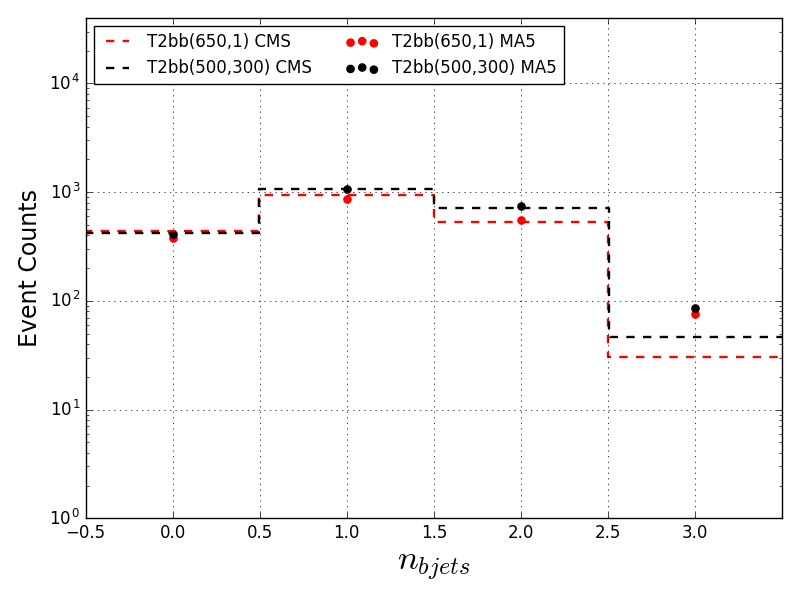
\includegraphics[width=0.49\textwidth]{PLOTS/Sbottoms_bJets_Pre.png}}
\subfigure {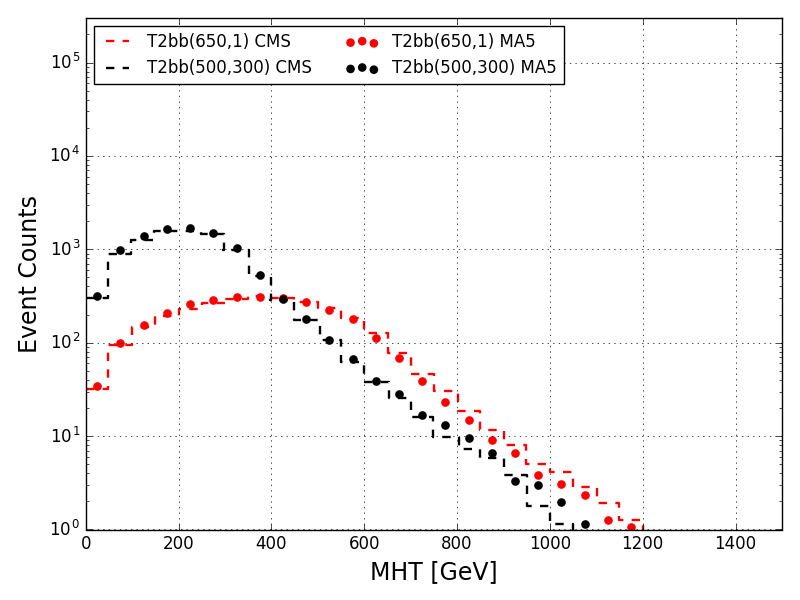
\includegraphics[width=0.49\textwidth]{PLOTS/Sbottoms_MHT_Pre.png}}
\subfigure {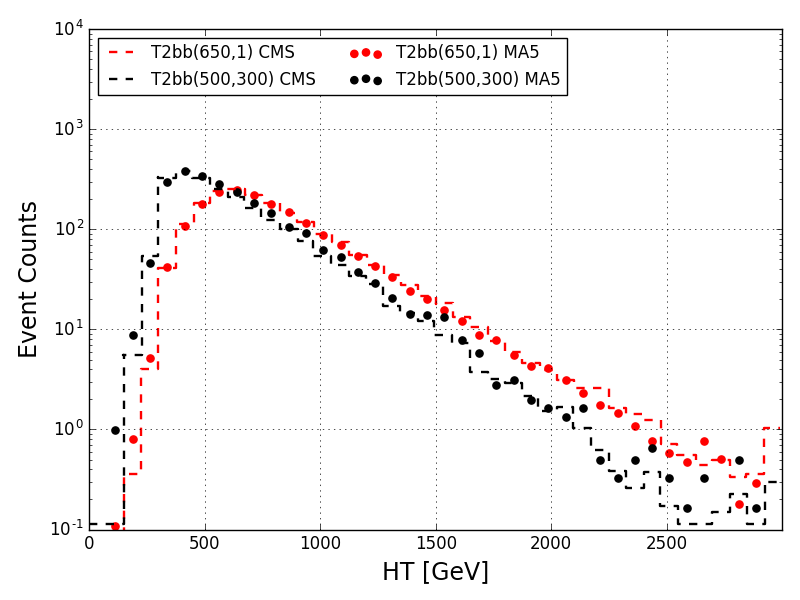
\includegraphics[width=0.49\textwidth]{PLOTS/Sbottoms_HT_Pre.png}}
\subfigure {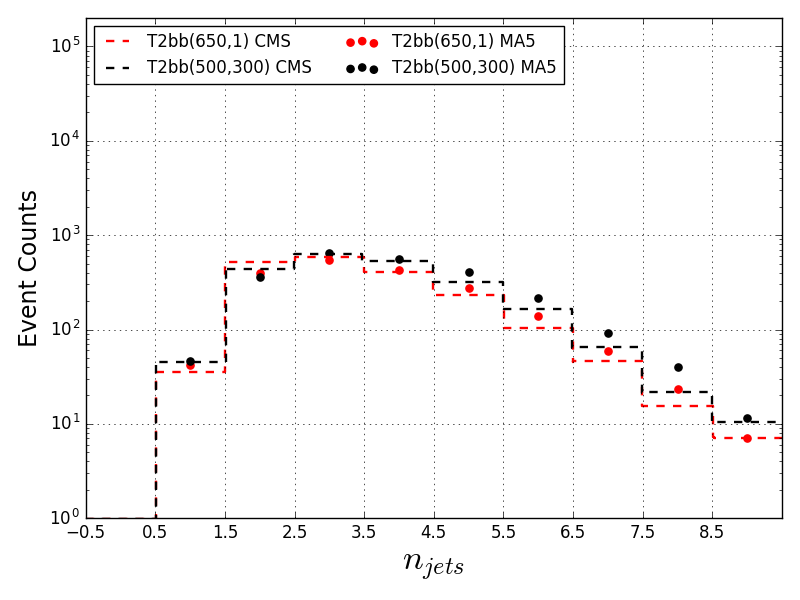
\includegraphics[width=0.49\textwidth]{PLOTS/Sbottoms_nJets_Pre.png}}
\end{center}
\caption{Kinematic distributions for the T2bb simplified models.}
\end{figure}

\clearpage
\begin{table}
\renewcommand{\arraystretch}{1.5}
\centering
\scriptsize
\begin{tabular} {  c | c | c | c | c | c  ||  c | c | c | c | c  }  
\multicolumn{1}{ c }{ }  &  \multicolumn{5}{ c }{ \textbf{T2bb(500,300)}} & \multicolumn{5 }{c}{ \textbf{T2bb(650,1)}} \\ \toprule
 \multicolumn{1}{ c }{ } &  \multicolumn{3}{c}{Absolute} & \multicolumn{2}{c}{Drop[$\%$]} & \multicolumn{3}{c}{Absolute} & \multicolumn{2}{c}{Drop[$\%$]} \\ \toprule \toprule
 \textbf{Cut} & \textbf{MA5} & \textbf{CMS} & \textbf{Diff(}\%\textbf{)} & \textbf{MA5} & \textbf{CMS} & \textbf{MA5} & \textbf{CMS} & \textbf{Diff(}\%\textbf{)} & \textbf{MA5} & \textbf{CMS} \\ \toprule \toprule

\NJETS~$\ge2$ &  95.27 & 96.00 & 0.76 & -4.73 & -4.00 &  97.36 & 98.20 & 0.85 & -2.64 & -1.80\\ 
\HT~$>$300 &  67.99 & 68.00 & 0.02 & -28.64 & -29.17 &  94.17 & 95.40 & 1.29 & -3.27 & -2.85\\ 
\MHT~$>$300 &  14.89 & 15.60 & 4.53 & -78.09 & -77.06 &  56.99 & 59.80 & 4.70 & -39.49 & -37.32\\ 
NoIsoMuons &  14.89 & 15.60 & 4.56 & -0.03 & 0.00 &  56.98 & 59.60 & 4.39 & -0.01 & -0.33\\ 
NoMuonsTracks &  14.87 & 15.50 & 4.03 & -0.10 & -0.64 &  56.94 & 59.50 & 4.31 & -0.08 & -0.17\\ 
NoIsoElectrons &  14.87 & 15.40 & 3.42 & -0.01 & -0.65 &  56.94 & 59.20 & 3.82 & 0.00 & -0.50\\ 
NoElectronsTracks &  14.85 & 15.30 & 2.95 & -0.17 & -0.65 &  56.90 & 59.00 & 3.56 & -0.06 & -0.34\\ 
NoIsoTracks &  14.79 & 15.20 & 2.67 & -0.37 & -0.65 &  56.70 & 58.50 & 3.07 & -0.35 & -0.85\\ 
$\Delta \phi(\vec{\slashed{H_T}},\vec{j_1})>$0.5 &  14.77 & 15.10 & 2.21 & -0.19 & -0.66 &  56.62 & 58.40 & 3.06 & -0.15 & -0.17\\ 
$\Delta \phi(\vec{\slashed{H_T}},\vec{j_2})>$0.5 &  13.84 & 14.10 & 1.86 & -6.29 & -6.62 &  54.15 & 55.70 & 2.78 & -4.35 & -4.62\\ 
$\Delta \phi(\vec{\slashed{H_T}},\vec{j_3})>$0.3 &  13.34 & 13.50 & 1.22 & -3.63 & -4.26 &  51.66 & 53.30 & 3.07 & -4.59 & -4.31\\ 
$\Delta \phi(\vec{\slashed{H_T}},\vec{j_4})>$0.3 &  12.57 & 13.10 & 4.07 & -5.76 & -2.96 &  49.09 & 51.60 & 4.87 & -4.99 & -3.19\\ 
\bottomrule \bottomrule
\end{tabular}
\caption{Pre-selection cutflow for the \textit{T2bb} simplified model.}
\end{table}


\begin{table} 
\scriptsize
\renewcommand{\arraystretch}{1.5}
\centering
\begin{tabular}{ c || c | c || c | c } 
\multicolumn{1}{c}{}   & \multicolumn{2}{ c }{ \textbf{T2bb(500,300)}} & \multicolumn{2}{c}{ \textbf{T2bb(650,1)}} \\ \toprule
 \textbf{Aggregated Signal Region} & \textbf{MA5} & \textbf{CMS}  & \textbf{MA5} & \textbf{CMS} \\ \toprule \toprule 
SR1-Njet2-Nb0-HT500-MHT500 &  57.91 & 50.48 & 145.59 & 168.10\\  
SR2-Njet3-Nb0-HT1500-MHT750 &  1.32 & 1.46 & 2.87 & 3.57\\  
SR3-Njet5-Nb0-HT500-MHT-500 &  20.29 & 18.32 & 32.71 & 32.40\\  
SR4-Njet5-Nb0-HT1500-MHT750 &  0.82 & 0.95 & 1.82 & 1.65\\  
SR5-Njet9-Nb0-HT1500-MHT750 &  0.00 & 0.10 & 0.22 & 0.08\\  
SR6-Njet2-Nb2-HT500-MHT500 &  98.67 & 86.76 & 224.70 & 202.30\\  
SR7-Njet3-Nb1-HT750-MHT750 &  29.53 & 24.11 & 41.93 & 47.20\\  
SR8-Njet5-Nb3-HT500-MHT500 &  10.56 & 5.54 & 17.28 & 6.90\\  
SR9-NJet5-Nb2-HT1500-MHT750 &  3.63 & 2.02 & 3.19 & 2.30\\  
SR10-Njet9-Nb3-HT750-MHT750 &  0.00 & 0.06 & 0.22 & 0.08\\  
SR11-Njet7-Nb1-HT300-MHT300 &  128.86 & 80.14 & 79.62 & 57.00\\  
SR12-Njet5-Nb1-HT750-MHT750 &  17.16 & 12.35 & 19.71 & 19.57\\  
\bottomrule \bottomrule
\end{tabular}
\caption{Yields in the aggregated signal regions for the \textit{T2bb} simplified model.}
\end{table}

\clearpage
\subsection{T1qqqq Simplified Model}
\begin{figure}[ht!] \begin{center}
\subfigure {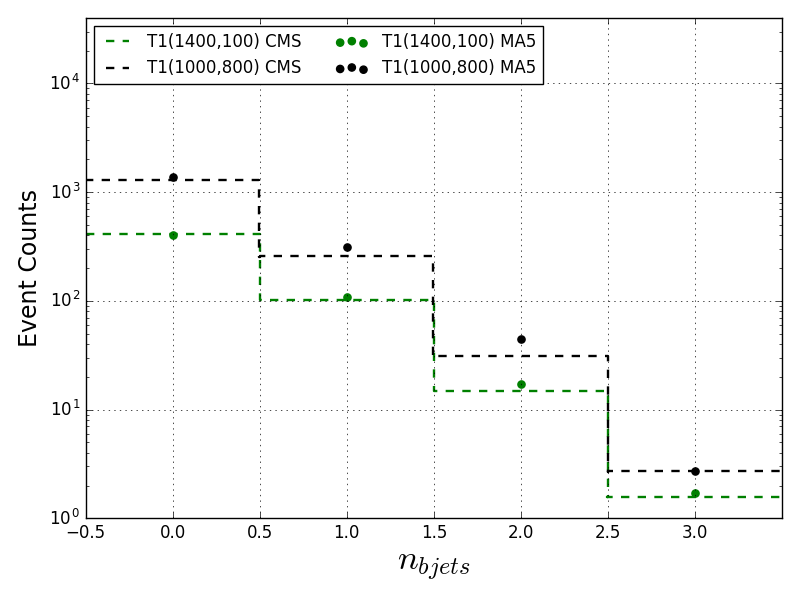
\includegraphics[width=0.49\textwidth]{PLOTS/T1qqqq_bJets_Pre.png}}
\subfigure {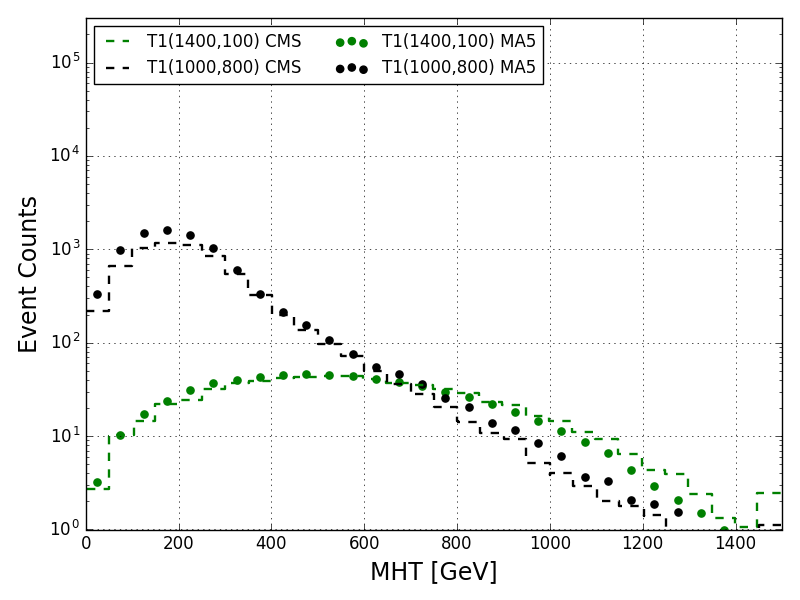
\includegraphics[width=0.49\textwidth]{PLOTS/T1qqqq_MHT_Pre.png}}
\subfigure {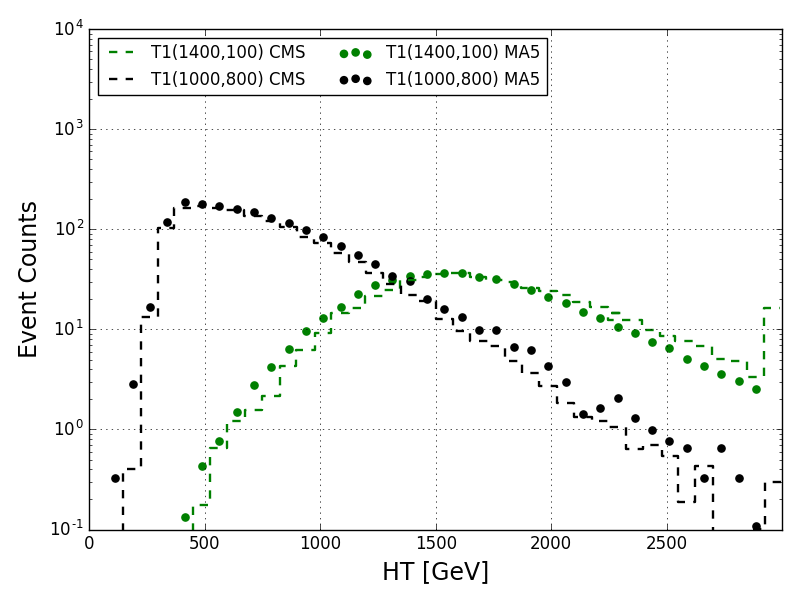
\includegraphics[width=0.49\textwidth]{PLOTS/T1qqqq_HT_Pre.png}}
\subfigure {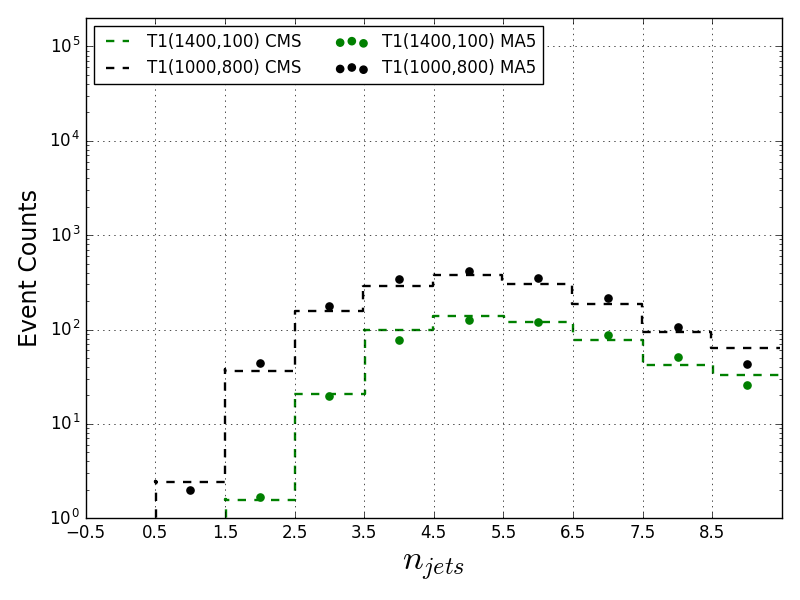
\includegraphics[width=0.49\textwidth]{PLOTS/T1qqqq_nJets_Pre.png}}
\end{center}
\caption{Kinematic distributions for the T1qqqq simplified models.}
\end{figure}

\clearpage
\begin{table}
\renewcommand{\arraystretch}{1.5}
\centering
\scriptsize
\begin{tabular} {  c | c | c | c | c | c  ||  c | c | c | c | c  }  
\multicolumn{1}{ c }{ }  &  \multicolumn{5}{ c }{ \textbf{T1qqqq(1000,800)}} & \multicolumn{5 }{c}{ \textbf{T1qqqq(1400,100)}} \\ \toprule
 \multicolumn{1}{ c }{ } &  \multicolumn{3}{c}{Absolute} & \multicolumn{2}{c}{Drop[$\%$]} & \multicolumn{3}{c}{Absolute} & \multicolumn{2}{c}{Drop[$\%$]} \\ \toprule \toprule
 \textbf{Cut} & \textbf{MA5} & \textbf{CMS} & \textbf{Diff(}\%\textbf{)} & \textbf{MA5} & \textbf{CMS} & \textbf{MA5} & \textbf{CMS} & \textbf{Diff(}\%\textbf{)} & \textbf{MA5} & \textbf{CMS} \\ \toprule \toprule
 
\NJETS~$\ge2$ &  99.42 & 99.60 & 0.18 & -0.58 & -0.40 &  99.99 & 100.00 & 0.01 & -0.01 & 0.00\\  
\HT~$>$300 &  74.80 & 81.30 & 8.00 & -24.77 & -18.37 &  99.98 & 100.00 & 0.02 & -0.02 & 0.00\\  
\MHT~$>$300 &  14.30 & 19.10 & 25.11 & -80.88 & -76.51 &  77.79 & 80.00 & 2.77 & -22.20 & -20.00\\  
NoIsoMuons &  14.30 & 19.10 & 25.11 & 0.00 & 0.00 &  77.79 & 80.00 & 2.77 & 0.00 & 0.00\\  
NoMuonsTracks &  14.30 & 19.10 & 25.14 & -0.04 & 0.00 &  77.78 & 79.90 & 2.66 & -0.01 & -0.12\\  
NoIsoElectrons &  14.30 & 19.00 & 24.75 & 0.00 & -0.52 &  77.78 & 79.50 & 2.17 & -0.00 & -0.50\\  
NoElectronsTracks &  14.29 & 18.80 & 23.99 & -0.06 & -1.05 &  77.76 & 79.10 & 1.69 & -0.02 & -0.50\\  
NoIsoTracks &  14.13 & 18.40 & 23.23 & -1.15 & -2.13 &  77.41 & 78.30 & 1.13 & -0.45 & -1.01\\  
$\Delta \phi(\vec{\slashed{H_T}},\vec{j_1})>$0.5 &  14.10 & 16.90 & 16.59 & -0.21 & -8.15 &  76.16 & 76.90 & 0.96 & -1.62 & -1.79\\  
$\Delta \phi(\vec{\slashed{H_T}},\vec{j_2})>$0.5 &  12.78 & 15.80 & 19.13 & -9.36 & -6.51 &  69.28 & 69.80 & 0.75 & -9.03 & -9.23\\  
$\Delta \phi(\vec{\slashed{H_T}},\vec{j_3})>$0.3 &  11.94 & 14.80 & 19.30 & -6.53 & -6.33 &  64.30 & 64.40 & 0.16 & -7.19 & -7.74\\  
$\Delta \phi(\vec{\slashed{H_T}},\vec{j_4})>$0.3 &  10.94 & 14.60 & 25.04 & -8.36 & -1.35 &  58.43 & 59.40 & 1.63 & -9.12 & -7.76\\  
\bottomrule
\end{tabular}
\caption{Pre-selection cutflow for the \textit{T1qqqq} simplified model.}
\end{table}


\begin{table} 
\scriptsize
\centering
\renewcommand{\arraystretch}{1.5}
\begin{tabular}{ c || c | c || c | c} 
\multicolumn{1}{c}{}   & \multicolumn{2}{ c }{ \textbf{T1qqqq(1000,800)}} & \multicolumn{2}{c}{ \textbf{T1qqqq(1400,100)}} \\ \toprule
 \textbf{Aggregated Signal Region} & \textbf{MA5} & \textbf{CMS}  & \textbf{MA5} & \textbf{CMS} \\ \toprule \toprule
 
 Aggregated Signal Region & MA5 & CMS  & MA5 & CMS \\  
SR1-Njet2-Nb0-HT500-MHT500 &  238.50 & 272.50 & 270.35 & 284.40\\  
SR2-Njet3-Nb0-HT1500-MHT750 &  20.33 & 18.79 & 72.06 & 88.90\\  
SR3-Njet5-Nb0-HT500-MHT-500 &  187.56 & 219.10 & 215.10 & 213.30\\  
SR4-Njet5-Nb0-HT1500-MHT750 &  18.87 & 17.51 & 61.38 & 69.90\\  
SR5-Njet9-Nb0-HT1500-MHT750 &  3.64 & 3.06 & 7.17 & 5.83\\  
SR6-Njet2-Nb2-HT500-MHT500 &  9.96 & 9.42 & 12.71 & 11.20\\  
SR7-Njet3-Nb1-HT750-MHT750 &  18.22 & 15.89 & 35.50 & 37.43\\  
SR8-Njet5-Nb3-HT500-MHT500 &  0.65 & 0.81 & 1.19 & 1.05\\  
SR9-NJet5-Nb2-HT1500-MHT750 &  0.81 & 0.94 & 3.21 & 3.49\\  
SR10-Njet9-Nb3-HT750-MHT750 &  0.00 & 0.07 & 0.10 & 0.12\\  
SR11-Njet7-Nb1-HT300-MHT300 &  76.77 & 87.10 & 52.18 & 42.97\\  
SR12-Njet5-Nb1-HT750-MHT750 &  15.47 & 14.07 & 29.97 & 30.67\\  
\bottomrule \bottomrule
\end{tabular}
\caption{Yield in the aggregated signal region for the \textit{T1qqqq} simplified model.}
\end{table}




\clearpage
\subsection{T1bbbb Simplified Model}
\begin{figure}[ht!] \begin{center}
\subfigure {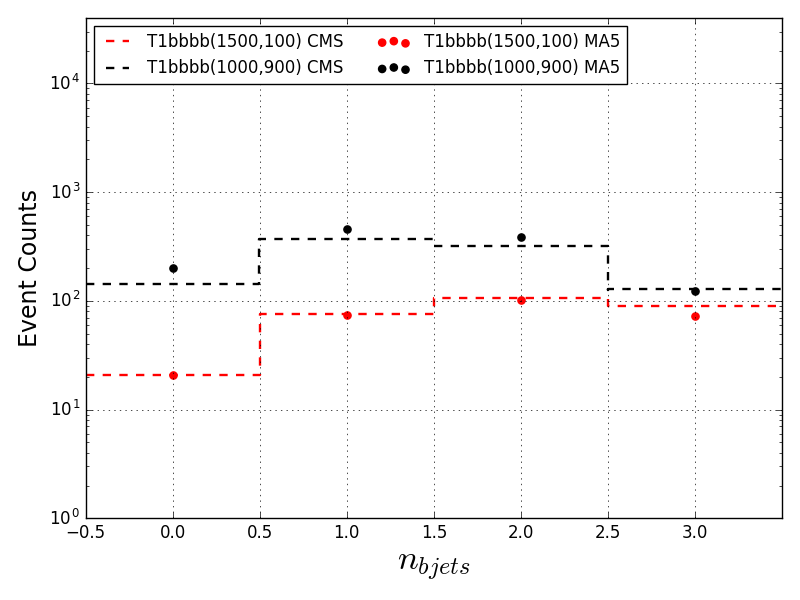
\includegraphics[width=0.49\textwidth]{PLOTS/T1bbbb_bJets_Pre.png}}
\subfigure {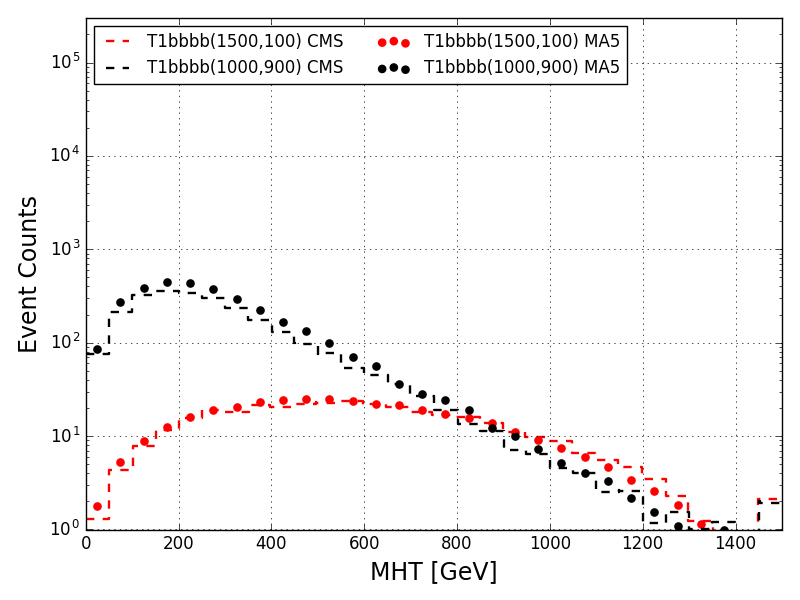
\includegraphics[width=0.49\textwidth]{PLOTS/T1bbbb_MHT_Pre.png}}
\subfigure {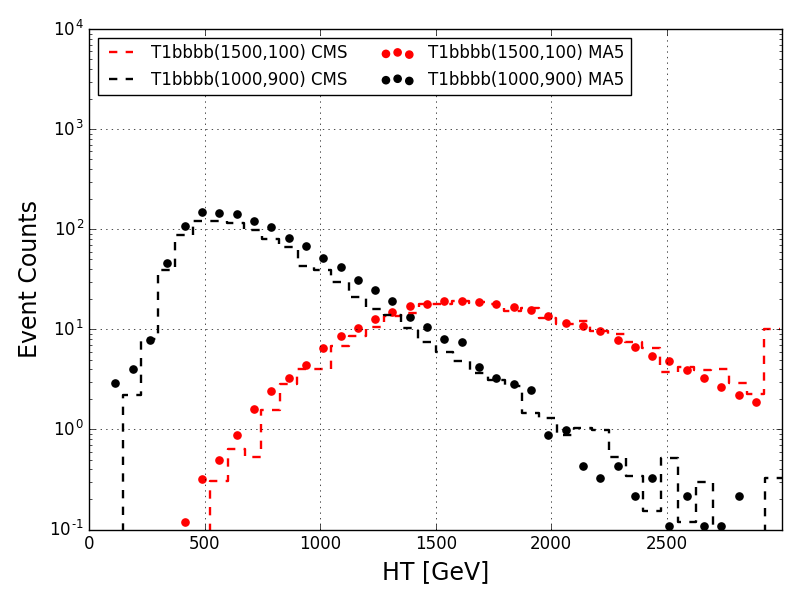
\includegraphics[width=0.49\textwidth]{PLOTS/T1bbbb_HT_Pre.png}}
\subfigure {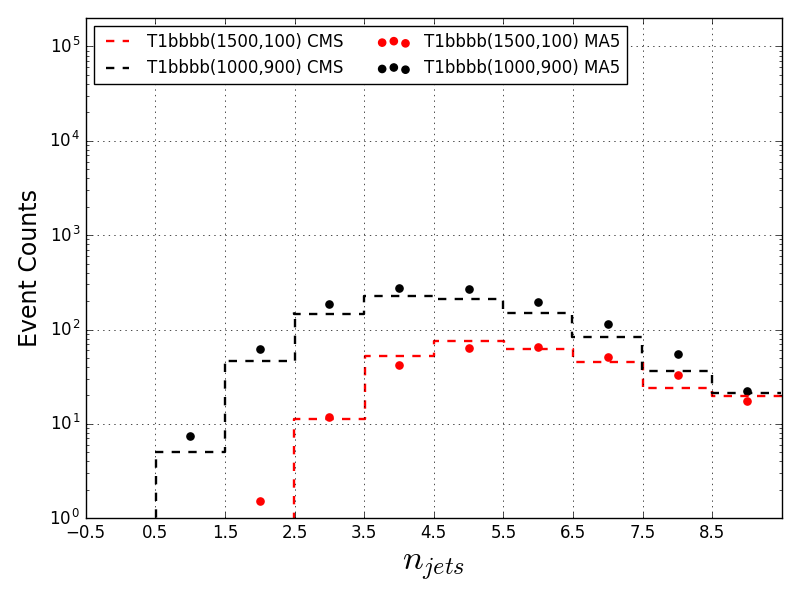
\includegraphics[width=0.49\textwidth]{PLOTS/T1bbbb_nJets_Pre.png}}
\end{center}
\caption{Kinematic distributions for the T1bbbb simplified models.}
\end{figure}

\clearpage
\begin{table}
\renewcommand{\arraystretch}{1.5}
\centering
\scriptsize
%\begin{tabular} {  c | l| l | l | l | l  ||  l | l | l | l | l  }  
\begin{tabular} {  c | c | c | c | c | c  ||  c | c | c | c | c  }  
\multicolumn{1}{ c }{ }  &  \multicolumn{5}{ c } {  \textbf{T1bbbb(1000,900)}} & \multicolumn{5 }{c}    {\textbf{T1bbbb(1500,100)}} \\ \toprule
 \multicolumn{1}{ c }{ } &  \multicolumn{3}{c}{Absolute} & \multicolumn{2}{c}{Drop[$\%$]} & \multicolumn{3}{c}{Absolute} & \multicolumn{2}{c}{Drop[$\%$]} \\ \toprule \toprule
 \textbf{Cut} & \textbf{MA5} & \textbf{CMS} & \textbf{Diff(}\%\textbf{)} & \textbf{MA5} & \textbf{CMS} & \textbf{MA5} & \textbf{CMS} & \textbf{Diff(}\%\textbf{)} & \textbf{MA5} & \textbf{CMS} \\ \toprule \toprule
 
\NJETS~$\ge2$ &  91.40 & 92.50 & 1.19 & -8.60 & -7.50 &  99.97 & 100.00 & 0.03 & -0.03 & 0.00\\  
\HT~$>$300 &  39.88 & 38.60 & -3.32 & -56.36 & -58.27 &  99.95 & 100.00 & 0.05 & -0.02 & 0.00\\  
\MHT~$>$300 &  14.32 & 14.10 & -1.57 & -64.09 & -63.47 &  79.36 & 80.30 & 1.17 & -20.60 & -19.70\\  
NoIsoMuons &  14.31 & 13.90 & -2.93 & -0.10 & -1.42 &  79.36 & 79.80 & 0.55 & -0.01 & -0.62\\  
NoMuonsTracks &  14.06 & 13.60 & -3.35 & -1.76 & -2.16 &  79.27 & 79.60 & 0.42 & -0.12 & -0.25\\  
NoIsoElectrons &  14.06 & 13.40 & -4.90 & 0.00 & -1.47 &  79.26 & 79.20 & -0.08 & -0.01 & -0.50\\  
NoElectronsTracks &  13.84 & 13.10 & -5.62 & -1.56 & -2.24 &  79.19 & 78.80 & -0.49 & -0.10 & -0.51\\  
NoIsoTracks &  13.75 & 12.80 & -7.40 & -0.65 & -2.29 &  78.90 & 78.00 & -1.15 & -0.37 & -1.02\\  
$\Delta \phi(\vec{\slashed{H_T}}$,$\vec{j_1})>$0.5 &  13.74 & 12.80 & -7.31 & -0.08 & 0.00 &  77.49 & 76.70 & -1.03 & -1.78 & -1.67\\  
$\Delta \phi(\vec{\slashed{H_T}}$,$\vec{j_2})>$0.5 &  12.19 & 11.40 & -6.94 & -11.24 & -10.94 &  70.38 & 69.20 & -1.70 & -9.18 & -9.78\\  
$\Delta \phi(\vec{\slashed{H_T}}$,$\vec{j_3})>$0.3 &  11.13 & 10.40 & -7.00 & -8.73 & -8.77 &  65.22 & 63.90 & -2.06 & -7.33 & -7.66\\  
$\Delta \phi(\vec{\slashed{H_T}}$,$\vec{j_4})>$0.3 &  10.28 & 9.60 & -7.11 & -7.59 & -7.69 &  59.15 & 58.60 & -0.94 & -9.30 & -8.29\\  
\bottomrule \bottomrule
\end{tabular}
\caption{Pre-selection cutflow for the \textit{T1bbbb} simplified model.}
\end{table}



\begin{table} 
\scriptsize
\renewcommand{\arraystretch}{1.5}
\centering
\begin{tabular}{ l || c | c || c | c } 
\multicolumn{1}{c}{}   & \multicolumn{2}{ c } {  \textbf{T1bbbb(1000,900)}} & \multicolumn{2}{c}{ \textbf{T1bbbb(1500,100)}} \\ \toprule
 \textbf{Aggregated Signal Region} & \textbf{MA5} & \textbf{CMS}  & \textbf{MA5} & \textbf{CMS} \\ \toprule \toprule
 
SR1-Njet2-Nb0-HT500-MHT500 &  66.94 & 46.90 & 14.41 & 14.68\\  
SR2-Njet3-Nb0-HT1500-MHT750 &  3.05 & 2.19 & 4.59 & 5.15\\  
SR3-Njet5-Nb0-HT500-MHT-500 &  28.45 & 18.40 & 9.76 & 9.75\\  
SR4-Njet5-Nb0-HT1500-MHT750 &  2.73 & 1.49 & 3.56 & 3.74\\  
SR5-Njet9-Nb0-HT1500-MHT750 &  0.65 & 0.15 & 0.39 & 0.28\\  
SR6-Njet2-Nb2-HT500-MHT500 &  173.45 & 138.65 & 141.44 & 137.51\\  
SR7-Njet3-Nb1-HT750-MHT750 &  76.31 & 63.07 & 89.04 & 93.83\\  
SR8-Njet5-Nb3-HT500-MHT500 &  43.83 & 34.77 & 62.94 & 52.78\\  
SR9-NJet5-Nb2-HT1500-MHT750 &  10.57 & 9.68 & 40.87 & 40.20\\  
SR10-Njet9-Nb3-HT750-MHT750 &  1.85 & 1.10 & 4.95 & 2.69\\  
SR11-Njet7-Nb1-HT300-MHT300 &  190.24 & 133.21 & 110.48 & 82.60\\  
SR12-Njet5-Nb1-HT750-MHT750 &  53.64 & 43.87 & 72.73 & 71.37\\  
\bottomrule \bottomrule
\end{tabular}
\caption{Aggregated signal region yields for the \textit{T1bbbb} simplified model.}
\end{table}


\clearpage
\section{Conclusion}
\normalsize
We presented the validation note for the analysis CMS-SUS-16-033. Overall the results look in good agreement with the official public data provided by the CMS collaboration, especially for the pre-selection cutflows, which show an agreement at the level of $O(\%)$.  
Deviations in the signal yields in the aggregated signal regions comparison can be noted especially in the regions where the tails of the distributions are considered. Note however that the largest differences are found for SR where the simulation details, e.g. Monte Carlo parameters and detector simulation efficiencies, are important, for example in the  bins of large \NJETS~and $N_{bjet}$ distributions. 
\\
\noindent




%
\begin{thebibliography}{9}


  
  %\cite{Conte:2012fm}
\bibitem{Conte:2012fm}
  E.~Conte, B.~Fuks and G.~Serret,
  %``MadAnalysis 5, A User-Friendly Framework for Collider Phenomenology,''
  Comput.\ Phys.\ Commun.\  {\bf 184} (2013) 222
  doi:10.1016/j.cpc.2012.09.009
  [arXiv:1206.1599 [hep-ph]].
  %%CITATION = doi:10.1016/j.cpc.2012.09.009;%%
  %232 citations counted in INSPIRE as of 17 Jul 2018
  
\bibitem{Conte:2014zja}
E.~Conte, B.~Dumont, B.~Fuks, and C.~Wymant, ``{Designing and recasting LHC
  analyses with MadAnalysis 5},'' {\em Eur. Phys. J.} {\bf C74} (2014), no.~10,
  3103,
\href{http://www.arXiv.org/abs/1405.3982}{{\tt 1405.3982}}.
%%CITATION = ARXIV:1405.3982;%%.

\bibitem{Dumont:2014tja}
B.~Dumont, B.~Fuks, S.~Kraml, S.~Bein, G.~Chalons, E.~Conte, S.~Kulkarni,
  D.~Sengupta, and C.~Wymant, ``{Toward a public analysis database for LHC new
  physics searches using MADANALYSIS 5},'' {\em Eur. Phys. J.} {\bf C75}
  (2015), no.~2, 56,
\href{http://www.arXiv.org/abs/1407.3278}{{\tt 1407.3278}}.
%%CITATION = ARXIV:1407.3278;%%.

%\cite{Sirunyan:2017cwe}
\bibitem{Sirunyan:2017cwe}
  A.~M.~Sirunyan {\it et al.} [CMS Collaboration],
  %``Search for supersymmetry in multijet events with missing transverse momentum in proton-proton collisions at 13 TeV,''
  arXiv:1704.07781 [hep-ex].
  %%CITATION = ARXIV:1704.07781;%%
  %1 citations counted in INSPIRE as of 23 May 2017
  
  
  %\cite{}
\bibitem{code}
  F.~Ambrogi and J.~Sonneveld,
  %``MadAnalysis5 recast of CMS-SUS-16-033,''
  doi:10.7484/INSPIREHEP.DATA.77YH.NBR3
  %%CITATION = doi:10.7484/INSPIREHEP.DATA.77YH.NBR3;%%
  
  
%\cite{Alwall:2011uj}
\bibitem{Alwall:2011uj}
  J.~Alwall, M.~Herquet, F.~Maltoni, O.~Mattelaer and T.~Stelzer,
  %``MadGraph 5 : Going Beyond,''
  JHEP {\bf 1106} (2011) 128
  doi:10.1007/JHEP06(2011)128
  [arXiv:1106.0522 [hep-ph]].
  %%CITATION = doi:10.1007/JHEP06(2011)128;%%
  %2694 citations counted in INSPIRE as of 17 Jul 2018
  
\bibitem{Alwall:2014hca}
J.~Alwall, R.~Frederix, S.~Frixione, V.~Hirschi, F.~Maltoni, O.~Mattelaer,
  H.~S. Shao, T.~Stelzer, P.~Torrielli, and M.~Zaro, ``{The automated
  computation of tree-level and next-to-leading order differential cross
  sections, and their matching to parton shower simulations},'' {\em JHEP} {\bf
  07} (2014) 079,
\href{http://www.arXiv.org/abs/1405.0301}{{\tt 1405.0301}}.
%%CITATION = ARXIV:1405.0301;%%.

%\cite{Sjostrand:2006za}
\bibitem{Sjostrand:2006za}
  T.~Sjostrand, S.~Mrenna and P.~Z.~Skands,
  %``PYTHIA 6.4 Physics and Manual,''
  JHEP {\bf 0605} (2006) 026
  doi:10.1088/1126-6708/2006/05/026
  [hep-ph/0603175].
  %%CITATION = doi:10.1088/1126-6708/2006/05/026;%%
  %9608 citations counted in INSPIRE as of 08 Aug 2018
  
  
%\cite{deFavereau:2013fsa}
\bibitem{deFavereau:2013fsa}
  J.~de Favereau {\it et al.} [DELPHES 3 Collaboration],
  %``DELPHES 3, A modular framework for fast simulation of a generic collider experiment,''
  JHEP {\bf 1402} (2014) 057
  doi:10.1007/JHEP02(2014)057
\href{http://www.arXiv.org/abs/arXiv:1307.6346}{{\tt 1307.6346}}
  %%CITATION = doi:10.1007/JHEP02(2014)057;%%
  %690 citations counted in INSPIRE as of 23 May 2017
  
  
\bibitem{Cacciari:2011ma}
M.~Cacciari, G.~P. Salam, and G.~Soyez, ``{FastJet User Manual},'' {\em
  Eur.Phys.J.} {\bf C72} (2012) 1896,
\href{http://www.arXiv.org/abs/1111.6097}{{\tt 1111.6097}}.
%%CITATION = ARXIV:1111.6097;%%.

\bibitem{Cacciari:2008gp}
M.~Cacciari, G.~P. Salam, and G.~Soyez, ``{The Anti-k(t) jet clustering
  algorithm},'' {\em JHEP} {\bf 0804} (2008) 063,
\href{http://www.arXiv.org/abs/0802.1189}{{\tt 0802.1189}}.
%%CITATION = ARXIV:0802.1189;%%.





\end{thebibliography}





\end{document}


